%
%==> Section: Drawing lines and curves
%
\section{
  Drawing lines and curves
}
%
%==> simple straight lines
%
\begin{frame}[fragile]
  \frametitle{
    Simples straight lines
  }
  To draw a line you do something like

  \lstinputlisting{./tex/src/draw_line.tex}
  
  and you get

  \begin{center}
    \begin{tikzpicture}
  \draw (0,0) --(1,2);
\end{tikzpicture}

  \end{center}
  
Ti$k$Z automatically draws a line between the points $(0,0)$ and $(1,2)$ and sets up the right space for the figure (by default, coordinates are in centimeters).
\end{frame}

%
%==> Sequence of segments
%
\begin{frame}

  You can do a sequence of segments which goes from point to point:

  \lstinputlisting{./tex/src/sequence_of_segments.tex}

  to get

  \begin{center}
    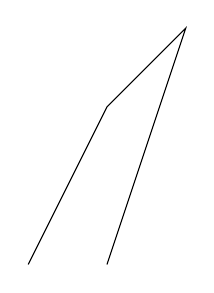
\begin{tikzpicture}
  \draw (0,0) --(1,2) -- (2,3) -- (1,0);
\end{tikzpicture}

  \end{center}
  
\end{frame}

%
%==> Add grid lines
%
\begin{frame}[fragile]

  We now have added the grid lines on the graphic to make it clearer. This is done through the command

  \begin{lstlisting}
    \draw[help lines] (0,0) grid (2,3);
  \end{lstlisting}

  which draws a grid from $(0,0)$ to $(2,3).$
  
  \lstinputlisting{./tex/src/add_grid_lines.tex}

  to get

  \begin{center}
    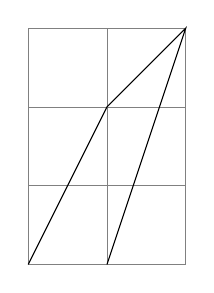
\begin{tikzpicture}
\draw[help lines] (0,0) grid (2,3);
\draw (0,0) --(1,2) -- (2,3) -- (1,0);
\end{tikzpicture}

  \end{center}

\end{frame}

%
%==> Add several lines
%
\begin{frame}[fragile]

  Of course, you can put several lines on the same graph:

  \lstinputlisting{./tex/src/add_several_lines.tex}

  yields

  \begin{center}
    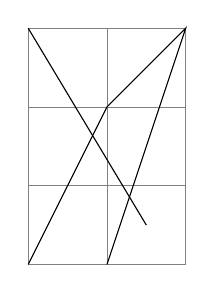
\begin{tikzpicture}
  \draw [help lines] (0,0) grid (2,3);
  \draw (0,0) --(1,2) -- (2,3) -- (1,0);
  \draw (0,3) -- (1.5,0.5);
\end{tikzpicture}

  \end{center}
  
  Notice the semi-colons ``; "at the end of lines -- they mark the end of instructions. That is, in the last picture we could have written

  {
    \footnotesize
    \begin{lstlisting}
      \draw (0,0) --(1,2) -- (2,3) -- (1,0); \draw (0,3) -- (1.5,0.5);
    \end{lstlisting}
  }
  
  without changing the output. You can also add and suppress spaces, for instance in order to make the code easier to read, without changing anything in the output.

\end{frame}

%
%==> Scaling pictures
%
\begin{frame}[fragile]
  \frametitle{
    Scaling pictures
  }

  One very useful feature of Ti$k$Z is that you can blow up the picture, by adding an option ``scale" to the environment.

  \begin{columns}
    \begin{column}{0.6\textwidth}
      \lstinputlisting{./tex/src/scaled_line.tex}
    \end{column}
    \begin{column}{0.4\textwidth}
      \begin{tikzpicture}[scale=2]
  \draw (0,0) -- (1,1);
\end{tikzpicture}

    \end{column}
  \end{columns}

  which you can compare to the following: 

  
  \begin{columns}
    \begin{column}{0.6\textwidth}
      \lstinputlisting{./tex/src/original_line.tex}
    \end{column}
    \begin{column}{0.4\textwidth}
      \begin{tikzpicture}
  \draw (0,0) -- (1,1);
\end{tikzpicture}

    \end{column}
  \end{columns}
  
\end{frame}
% Scaling in one dimension
\begin{frame}[containsverbatim]
You can scale only one dimension:

  \begin{columns}
    \begin{column}{0.6\textwidth}
      \lstinputlisting{./tex/src/scale_one_dimension.tex}
    \end{column}
    \begin{column}{0.4\textwidth}
      \begin{tikzpicture}[xscale=3]
  \draw (0,0) -- (1,1);
\end{tikzpicture}

    \end{column}
  \end{columns}


or both dimensions in different proportions:

  \begin{columns}
    \begin{column}{0.6\textwidth}
      \lstinputlisting{./tex/src/scale_both_dimensions.tex}
    \end{column}
    \begin{column}{0.4\textwidth}
      \begin{tikzpicture}[xscale=2.5,yscale=0.5]
  \draw (0,0) -- (1,1);
\end{tikzpicture}

    \end{column}
  \end{columns}

\end{frame}

%
%==> Arrows and the like
%
\begin{frame}[fragile]
  \frametitle{
    Arrows and the like
  }

  You can ``decorate" the lines. For instance we can put arrows or bars on one of both extremities:

  \lstinputlisting{./tex/src/decorate_lines.tex}
  
  which yields

  \begin{center}
    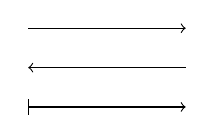
\begin{tikzpicture}
  \draw [->] (0,0) -- (2,0);
  \draw [<-] (0, -0.5) -- (2,-0.5);
  \draw [|->] (0,-1) -- (2,-1);
\end{tikzpicture}

  \end{center}
  
\end{frame}
%
%==> Coordinates
%
\begin{frame}[fragile]

  When you draw several segments, the arrows are placed at the extremities of the first and the last segments. This is convenient, among other things to draw axes (we will see later how to label them):

  \lstinputlisting{./tex/src/coordinates.tex}
  
which gives you

  \begin{center}
    \begin{tikzpicture}
  \draw [<->] (0,2) -- (0,0) -- (3,0);
\end{tikzpicture}

  \end{center}
  
\end{frame}
%
%==> Changing the thickness of lines
%
\begin{frame}[fragile]
  \frametitle{
    Changing the thickness of lines
  }

  Other decorations include changing the thickness:

  \lstinputlisting{./tex/src/change_line_thickness.tex}
  
  which gives you

  \begin{center}
    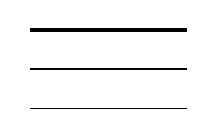
\begin{tikzpicture}
  \draw [ultra thick] (0,1) -- (2,1);
  \draw [thick] (0,0.5) -- (2,0.5);
  \draw [thin] (0,0) -- (2,0);
\end{tikzpicture}

  \end{center}
  
\end{frame}
%
%==> helplines
%
\begin{frame}[fragile]
  \frametitle{
    The help lines option
  }

  There is also the {\tt help lines} option, discussed earlier, which is made specially to be fine gray lines for showing special points:

    \lstinputlisting{./tex/src/add_help_lines.tex}
  
  which yields.

  \begin{center}
    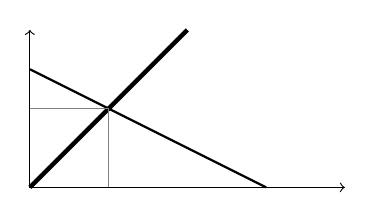
\begin{tikzpicture}
  \draw [<->] (0,2) -- (0,0) -- (4,0);
  \draw [thick] (0,1.5) -- (3,0);
  \draw [ultra thick] (0,0) -- (2,2);
  \draw [help lines] (1,0) -- (1,1) -- (0,1);
\end{tikzpicture}

  \end{center}
  
\end{frame}
%
%==> Custom line widths
%
\begin{frame}[fragile]
  \frametitle{
    Custom line widths
  }

  You can also use custom widths:

  \lstinputlisting{./tex/src/custom_line_widths.tex}
  
  which gives a line 12pt wide (the default dimension for width is point) and another one .2cm wide:

  \begin{center}
    
\begin{tikzpicture}
  \draw [line width=12] (0,0) -- (2,0);
  \draw [line width=0.2cm] (4,.75) -- (5,.25);
\end{tikzpicture}

  \end{center}
  
\end{frame}
%
%==> Dashes and dots
%
\begin{frame}[fragile]
  \frametitle{
    Dashes and dots
  }

  You can also make dashed and dotted lines

  \lstinputlisting{./tex/src/dashes_and_dots.tex}

  This gives:

    \begin{center}
    \begin{tikzpicture}
  \draw [dashed, ultra thick] (0,1) -- (5,1);
  \draw [dashed] (0, 0.5) -- (5,0.5);
  \draw [dotted] (0,0) -- (5,0);
\end{tikzpicture}

    \end{center}

    The top line shows you that you can mix types of decorations. You have lots of control over the style of your dotted and dashed lines (see the manual).

\end{frame}
%
%==> Colored lines
%
\begin{frame}[fragile]
  \frametitle{
    Colored lines
  }

  And finally, you can color your lines.

  \lstinputlisting{./tex/src/colored_lines.tex}

   We obtain

    \begin{center}
    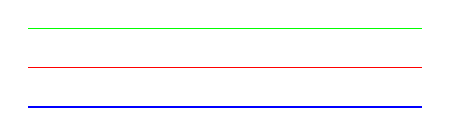
\begin{tikzpicture}
  \draw [green] (0,1) -- (5,1);
  \draw [red] (0, 0.5) -- (5,0.5);
  \draw [blue] (0,0) -- (5,0);
\end{tikzpicture}

    \end{center}

\end{frame}

%
%==> Taste the rainbow
%
\begin{frame}
  \frametitle{
    Taste the rainbow
  }
  You have direct access to the following pre-defined colors: red 
\begin{tikzpicture} \draw [red, line width=6]
     (0,0) -- (.5,0);  \end{tikzpicture}, 
green 
\begin{tikzpicture} \draw [green, line width=6]
     (0,0) -- (.5,0);  \end{tikzpicture}, blue 
\begin{tikzpicture} \draw [blue, line width=6]
     (0,0) -- (.5,0);  \end{tikzpicture}, cyan 
\begin{tikzpicture} \draw [cyan, line width=6]
     (0,0) -- (.5,0);  \end{tikzpicture}, magenta 
\begin{tikzpicture} \draw [magenta, line width=6]
     (0,0) -- (.5,0);  \end{tikzpicture}, yellow 
\begin{tikzpicture} \draw [yellow, line width=6]
     (0,0) -- (.5,0);  \end{tikzpicture}, black 
\begin{tikzpicture} \draw [black, line width=6]
     (0,0) -- (.5,0);  \end{tikzpicture}, darkgray\footnote{An affront to the King's language} 
\begin{tikzpicture} \draw [darkgray, line width=6]
     (0,0) -- (.5,0);  \end{tikzpicture}, light gray 
\begin{tikzpicture} \draw [lightgray, line width=6]
     (0,0) -- (.5,0);  \end{tikzpicture}, brown 
\begin{tikzpicture} \draw [brown, line width=6]
     (0,0) -- (.5,0);  \end{tikzpicture}, lime 
\begin{tikzpicture} \draw [lime, line width=6]
     (0,0) -- (.5,0);  \end{tikzpicture}, olive 
\begin{tikzpicture} \draw [olive, line width=6]
     (0,0) -- (.5,0);  \end{tikzpicture}, orange 
\begin{tikzpicture} \draw [orange, line width=6]
     (0,0) -- (.5,0);  \end{tikzpicture}, pink 
\begin{tikzpicture} \draw [pink, line width=6]
     (0,0) -- (.5,0);  \end{tikzpicture}, purple 
\begin{tikzpicture} \draw [purple, line width=6]
     (0,0) -- (.5,0);  \end{tikzpicture}, teal 
\begin{tikzpicture} \draw [teal, line width=6]
     (0,0) -- (.5,0);  \end{tikzpicture}, violet 
\begin{tikzpicture} \draw [violet, line width=6]
     (0,0) -- (.5,0);  \end{tikzpicture}, and white \begin{tikzpicture} \draw [white, line width=6]
  (0,0) -- (.5,0);  \end{tikzpicture}. And you can define all the colors you might want using the RGB color model (see the manual).
\end{frame}

%
%==> Pictures in the middle of text
%
\begin{frame}[fragile]
  \frametitle{
    Pictures in the middle of text
  }

  By the way, you may wonder how we included these rectangles in the text. Ti$k$Z makes a picture wherever 
\begin{tikzpicture}
  \draw [blue, line width=6] (0,0) -- (.5,0);
\end{tikzpicture}
 you want; we just typed

  \begin{center}
    \lstinputlisting{./tex/src/blue_in_middle_of_text.tex}
  \end{center}

  wherever we want in the text. To make these constructions easier to type you can use the command {\tt \bf \textbackslash tikz}  (see the manual).

\end{frame}

%
%==> Curves
%
\begin{frame}[fragile]
  \frametitle{
    Curves
  }

  We are not limited to straight lines:

  { \footnotesize
  \lstinputlisting{./tex/src/shapes.tex}
  }
  
  This gives:

  \begin{center}
    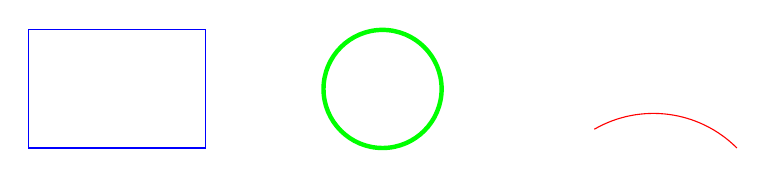
\begin{tikzpicture}[scale=1.5]
  \draw [blue] (0,0) rectangle (1.5,1);
  \draw [green, ultra thick] (3,0.5) circle [radius=0.5];
  \draw [red] (6,0) arc [radius=1, start angle=45, end angle= 120];
\end{tikzpicture}

  \end{center}

  The arc is of radius 1, starts at the point $(6,0)$ leaving it at an angle of $45^\circ$ and stops when its slope is $120^\circ$.

\end{frame}

%
%==> Smoother curves
%
\begin{frame}[fragile]
  \frametitle{
    Smoother curves
  }

  We can make paths take smoother turns:

  { \footnotesize
  \lstinputlisting{./tex/src/rounded_corners.tex}
  }
  
  which gives us

  \begin{center}
    \begin{tikzpicture}
  \draw [<->, rounded corners, thick, purple] (0,2) -- (0,0) -- (3,0);
\end{tikzpicture}

  \end{center}

\end{frame}
%
%==> Hard coding graphs
%
\begin{frame}[containsverbatim]
  \frametitle{
    Hard coding graphs
  }

  If you want a precise curve you can do it by computing lots of points in a program such as C/C++, Fortran, Python, MATLAB, etc, and then putting them into Ti$k$Z: 

  {
    \scriptsize
    \lstinputlisting{./tex/src/hard_coded_graph.tex}
  }
  
\end{frame}

%
%==> Hard coded graph results
%
\begin{frame}[containsverbatim]
    \frametitle{
    Hard coded graph results
    }

    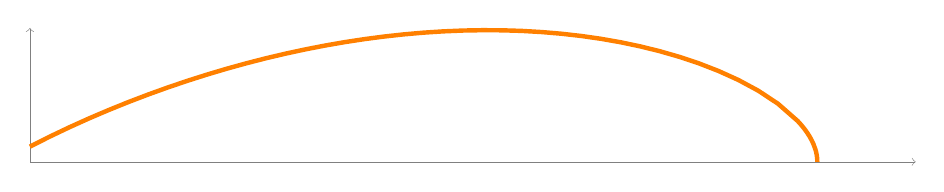
\begin{tikzpicture}[xscale=25,yscale=5]
  \draw [<->, help lines] (0.6,1.34) -- (0.6,1) -- (1.05,1);
  \draw [orange, ultra thick] (0.6, 1.0385) --
(0.61, 1.06372) -- (0.62, 1.08756) -- (0.63, 1.11012) -- (0.64,
1.13147) -- (0.65, 1.15166) -- (0.66, 1.17074) -- (0.67, 1.18874) -- (0.68,
1.20568) -- (0.69, 1.22157) -- (0.7, 1.23643) -- (0.71, 1.25026) -- (0.72,
1.26307) -- (0.73, 1.27486) -- (0.74, 1.28561) -- (0.75, 1.29534) -- (0.76,
1.30402) -- (0.77, 1.31165) -- (0.78, 1.31821) -- (0.79, 1.32369) -- (0.8,
1.32806) -- (0.81, 1.33131) -- (0.82, 1.3334) -- (0.83, 1.33431) -- (0.84,
1.334) -- (0.85, 1.33244) -- (0.86, 1.32956) -- (0.87, 1.32533) -- (0.88,
1.31966) -- (0.89, 1.3125) -- (0.9, 1.30373) -- (0.91, 1.29325) -- (0.92,
1.2809) -- (0.93, 1.26649) -- (0.94, 1.24976) -- (0.95, 1.23032) -- (0.96,
1.2076) -- (0.97, 1.18065) -- (0.98, 1.14763) -- (0.99, 1.1038) -- (0.991,
1.09836) -- (0.992, 1.09261) -- (0.993, 1.0865) -- (0.994, 1.07994) -- (0.995,
1.07282) -- (0.996, 1.06497) -- (0.997, 1.0561) -- (0.998, 1.04563) -- (0.999,
1.03209) -- (0.9991, 1.03042) -- (0.9992, 1.02866) -- (0.9993,
1.02679) -- (0.9994, 1.02478) -- (0.9995, 1.0226) -- (0.9996, 1.02019) -- (0.9997,
1.01747) -- (0.9998, 1.01424) -- (0.9999, 1.01005) -- (0.9999,
1.01005) -- (0.99991, 1.00953) -- (0.99992, 1.00898) -- (0.99993,
1.0084) -- (0.99994, 1.00778) -- (0.99995, 1.0071) -- (0.99996,
1.00634) -- (0.99997, 1.00549) -- (0.99998, 1.00448) -- (0.99999, 1.00317) -- (1,1);
\end{tikzpicture}


    \begin{enumerate}
    \item
      This was overkill: We do not need so many points;
    \item
      This can also serve as a reminder that one Ti$k$Z instruction can be spread over several lines and cut arbitrarily over several lines. The marker is the semi-colon, not the end of line!
    \end{enumerate}

\end{frame}

%
%==> Plot curve
%
\begin{frame}[fragile]

  There are a number of ways by which you can do curves without plotting all the points. Here is an easy one:

  \lstinputlisting{./tex/src/plot_curve.tex}
  
  This gives us a curve from $(0,0)$ to $(2,1.5)$ which leaves at an angle of $90^\circ$ and arrive at an angle of $195^\circ$: Notice that we replaced the \textcolor{red}{\tt  --} with \textcolor{red}{\tt to}.

  \begin{center}
    \begin{tikzpicture}[scale=3]
  \draw [very thick] (0,0) to [out=90,in=195] (2,1.5);
\end{tikzpicture}

  \end{center}
  
\end{frame}
%
%==> Replacing -- with to
%
\begin{frame}
  \frametitle{
    Replacing \textbf{\tt  --} with \textbf{\tt to}
  }

  \begin{center}
    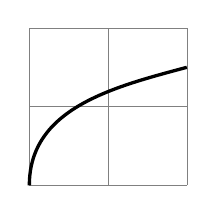
\begin{tikzpicture}
      \draw [style=help lines] (0,0) grid (2,2);
      \draw [very thick] (0,0) to [out=90,in=195] (2,1.5);
    \end{tikzpicture}
  \end{center}
  
  \begin{enumerate}
  \item
    When the curves goes \textcolor{red}{out} of $(0,0),$ you put a needle with one extremity on the starting point and the other one facing right and you turn it counterclockwise until it is tangent to the curve. The angle by which you have to turn the needle gives you the \textcolor{red}{out} angle.
  \item
    When the curves goes \textcolor{red}{in} at $(2,1.5),$ you put a needle with one extremity on the arrival point and the other one facing right and you turn it counterclockwise until it is tangent to the curve. The angle by which you have to turn the needle gives you the \textcolor{red}{in} angle.
  \end{enumerate}

\end{frame}

%
%==> Several to instructions
%
\begin{frame}[fragile]
  \frametitle{
    Several \textbf{\tt to} instructions
  }
  
  As with straight lines you can put several \textbf{\tt to} instructions in the same Ti$k$Z instruction:

  \lstinputlisting{./tex/src/several_to_instructions.tex}
  
  we obtain:

  \begin{center}
    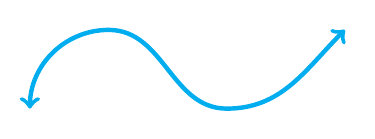
\begin{tikzpicture}
  \draw [<->,ultra thick, cyan]
  (0,0) to [out=90,in=180]
  (1,1) to [out=0,in=180]
  (2.5,0) to [out=0,in=-135] (4,1);
\end{tikzpicture}

  \end{center}
  
\end{frame}
